\documentclass[review]{elsarticle}

\usepackage[]{geometry}
\usepackage{amsmath}
\usepackage{amssymb}
\usepackage{graphicx}
\usepackage{xcolor}
\usepackage{hyperref}
\usepackage{natbib}
\bibliographystyle{elsarticle-harv}
\biboptions{authoryear}

\newcommand{\ra}{\rightarrow}
\newcommand{\afs}[2]{\Phi_{#1}^{(#2)}}
\newcommand{\Dfrac}[2]{%
  \ooalign{%
    $\genfrac{}{}{1.2pt}0{#1}{#2}$\cr%
    $\color{white}\genfrac{}{}{.4pt}0{\phantom{#1}}{\phantom{#2}}$}%
}
\newcommand{\cond}{\middle\vert}
\newcommand{\dslash}{/\!\!/}
\newcommand{\Coalc}[4]{\begin{bmatrix}#1\dslash #2 \\ #3\dslash #4 \end{bmatrix}}

\newcommand{\sgcomment}[1]{{\color{red}{SG: #1}}}
\newcommand{\ikcomment}[1]{{\color{blue}{IK: #1}}}
\newcommand{\Var}{\operatorname{Var}}
\journal{Theoretical Population Biology}

\begin{document}
\begin{frontmatter}
  \title{Models of strong selection in large samples}

  \author{Ivan Krukov}
  \author{Simon Gravel}

  \begin{abstract}
    Neutral models of genetic diversity tend to be easier to study than models including selection.
    In the Wright-Fisher model, the number of parental lineages that contribute to ancestry of a
    sample is lower than the number of offspring. As a consequence, useful recursion equations can
    be derived for patterns of polymorphism. By contrast, under negative selection, the number of
    relevant lineages can increase as we go back in time, due to selective deaths. As a result, the
    equivalent recursion equations do not close. However, given a sufficiently large sample size,
    the expected reduction in the number of contributing lineages due to coalescence is larger than
    the increase due to selection, so the net number is unlikely to increase. We use this
    observation to derive asymptotically closed recursion equations for the distribution of allele
    frequencies in finite samples. We show that this approach is accurate under strong drift and
    strong natural selection. We derive several asymptotic results to determine when the sample size
    is sufficiently large for drift to overcome the effect of selection.
  \end{abstract}

\end{frontmatter}

\section{Introduction}
\label{sec:introduciton}

The allele frequency spectrum (\textit{AFS}) is an important summary of genetic diversity that is
commonly used to infer demographic history and natural selection \citep{}. Given a demographic
scenario of population size histories and migrations, the diffusion approximation or coalescent
simulations can be used to obtain a predicted \textit{AFS} \citep{}. By comparing predictions to the
observed \textit{AFS}, one can compute likelihoods for different demographic scenarios.
Unfortunately, the \textit{AFS} calculations can be time consuming with complex demographic models,
for example with multiple populations, or with large sample sizes \citep{}.

In the absence of selection, efficient computational shortcuts can be used. In particular, recursion
equations have been derived for moments of the allele frequency distribution
\citep{KimuraCrow1964,Ewens1972,JouganousEtAl2017}. Recently, these recursions have been useful in
fitting complex demographic models to genetic data \citep{JouganousEtAl2017,KammEtAl2017}.
 
In the presence of natural selection, the corresponding recursion equations do not close
\citep{Donnelly, JouganousEtAl2017} -- they form an infinite set of coupled ordinary differential
equations. Moment-based closure approximation have been developed \citep{JouganousEtAl2017}, but
these are not robust to strong selection and their convergence properties are not well understood.

Closure of the moment equations under the neutral Wright-Fisher model occurs because the number of
parental lineages that contribute to the present day sample is equal to or smaller than the sample
size, which is due to coalescent events back in time \citep{Kingman1982a}. This does not hold under
negative selection -- due to selective deaths, the number of parental lineages that contribute can
be larger than the sample size, $n$. As we demonstrate later, this leads to a potentially infinite
number of terms in the equations. The potential increase in the number of relevant lineages as we go
back in time is explicit in the ancestral selection graphs (\textit{ASG}),
\citep{KroneNeuhauser1997}.

The actual increase in the number of lineages as we go back in time depends on the relative
importance of drift and selection. The number of coalescent events per generation is proportional to
the square of the sample size $n$, while the number of selective deaths is linear in $n$. This
suggests that with sufficiently large samples, the effect of selection would be smaller than that of
drift, which would prevent the increase in the number of lineages -- at least most of the times.
Thus recursion equations can become almost-closed, in a sense that we will explore below.

An additional complication is multiple and/or simultaneous coalescent events -- which emerge with
large sample sizes \citep{BhaskarEtAl2014}. The standard coalescent model only allows one event per
generation, but we also need to consider higher-order events, \textit{e.g.} multiple two-lineage or
three-lineage mergers. These multiple-lineage coalescent events oppose the effect of selection by
rapidly decreasing the number of contributing lineages \citep{NelsonEtAl2019}.

In this article we derive these asymptotically-closed recursions in the Wright-Fisher model, and
study their behaviour and applications for modelling the distribution of allele frequencies under
strong selection.

\section{Background}
\label{sec:background}

We consider a haploid Wright-Fisher model of size $N$, focusing on a single biallelic locus. For a
present-day sample with $n_o$ offspring lineages at time $t$, we will be looking for recursion
equations for the allele frequency spectrum ($\afs{n_o}{t}(i_o)$) by considering the sampling process
in a finite sample under drift and selection. We define the \textit{AFS} as a probability of
observing $i_o$ copies of the derived allele at a single locus in $n_o$ samples.

\begin{center}
  \label{Table of symbols}
\begin{tabular}{l|p{100mm}}
Symbol & Meaning\\
\hline
$N$ & Population size\\
$n_p$ & Number of parental lineages\\
$n_g$ & Number of gametes\\
$n_o$ & Number of offspring, sample size\\
$i_p$ & Number of derived alleles in parents\\
$i_o$ & Number of derived alleles in offspring\\
$t$ & Time, in generations\\
$\Phi_{n_o}^{t}(i_o)$ & Allele frequency spectrum in $n_o$ at generation $t$\\
$s$ & Selection advangate of the derived allele\\
$x$ & Frequency of derived allele at generation $t$\\
$i_o \dslash n_o$ & A sample with $i_o$ derived alleles ``out of'' $n_o$ total\\
 & \\
\end{tabular}
\end{center}

Under neutral evolution, the number of lineages in the sample decreases into the past due to
coalescent events (Fig.\ref{fig:schematic}A). Specifically, the parental generation carries $n_p$
alleles, and the offspring generation - $n_o$ alleles. Under neutrality $n_p \le n_o$.

Under selection, a lineage of a derived allele can be ``rejected'' as a result of selective death
(Fig. \ref{fig:schematic}B). To track the number of derived (deleterious) alleles, we introduce the
notation $i_p \dslash n_p$ to represent that $i_p$ alleles are derived ``out of'' total $n_p$
parental alleles. $i_o \dslash n_o$ represents the offspring generation.

In case of a selective death a lineage can be resampled, with probability $1-s$, leading to $1:1-s$
advantage of the ancestral allele. Under selection, it is possible that $n_p \ge n_o$. We use this
notation and model in section XX.

It is also convenient to make the number of gametes produced by the parental generation explicit
(Fig. \ref{fig:schematic}C). We denote the number of these intermediate gametes with $n_g$. In our
model, the production of gametes is neutral, thus $n_p \le n_g$. The assortment of gametes into the
offspring is subject to selection, so $n_g \ge n_o$. This two-step process allows us to consider
effects of drift and selection within a single generation. In the case where there is more
coalescent selection events, we can have $n_p \le n_o$. We use this observation in section XX.

\begin{figure}[ht]
  \centering
  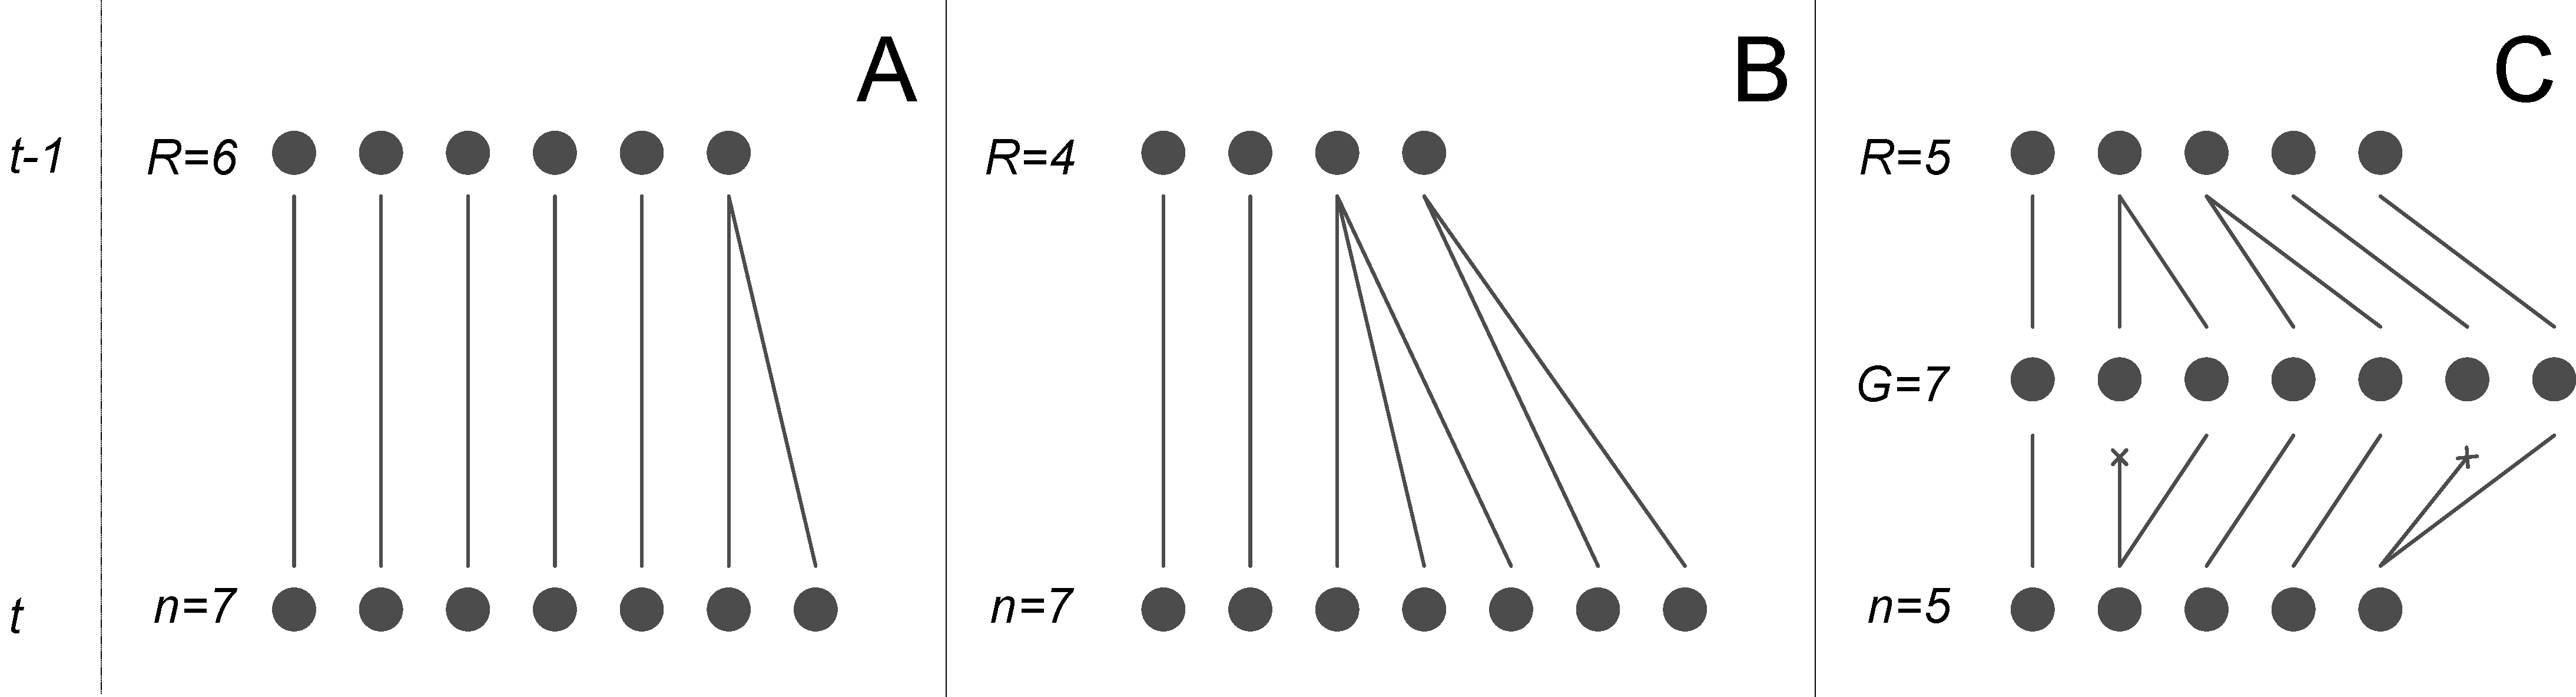
\includegraphics[width=1.0\textwidth]{fig/schematic.pdf}
  \caption{\label{fig:schematic} Realizations of sampling parental lineages under neutrality (A) and
    under selection (B,C). \textbf{A} Under neutrality, possible coalescent events imply that number
    of parental lineages $n_p$ at $t-1$ is less than or equal to $n_o$ offspring lineages at $t$.
    \textbf{B} With selection, re-sampling events are also possible, thus $n_p \ge n_o$. The net
    number of selection minus the coalescent events will indicate if the equations close. \textbf{C}
    It is also instructive to consider the number of gametes ($n_g$) produced. If we posit that
    production of gametes is neutral, and the passing of gametes to offspring is under the control
    of selection, we can develop a more intuitive understanding of the interplay of the two forces.
  }
\end{figure}

To express the allele-frequency spectrum $\afs{n_o}{t}$ for $n_o$ offspring in terms of the
\textit{AFS} at time $t-1$, we can sum over the random variables $n_p$, the number of distinct
contributing parental lineages selected, and $i_p$, the number of derived lineages among them:

\begin{equation}
\afs{n_o}{t}(i_o)=\sum_{n_p,i_p} P_{n_o}(i_o,i_p,n_p) = 
                  \sum_{n_p,i_p} P_{n_o}(i_o|i_p,n_p) P(i_p,n_p),
\end{equation}

where the subscript $n_o$ indicates probabilities that depend on $n_o$. The event $(i_p,n_p)$ means
that our Wright-Fisher sampling for $n_o$ offspring selected exactly $n_p$ distinct ancestors, of
which $i_c$ are derived. Under Wright-Fisher sampling, the order in which (previously unsampled)
parental lineages are drawn is random. That is, we could have performed a random permutation of the
parental population prior to starting the sampling process, and sampled new parental lineages in
order from this permutation. Thus the event $(i_c,n_p)$ can be reformulated as the joint events that
the first $n_p$ parental alleles from the random permutation carry $i_c$ derived alleles \textit{and}
that exactly $n_p$ distinct parents were drawn in the Wright-Fisher sampling of the first $n_o$
offspring. Now, let $r(i_c,n_p)$ be the (less specific) event that the first $n_p$ parental alleles
from the random permutation carry $i_c$ derived alleles. Then $P(r(i_c,n_p)) =\afs{n_p}{t} (i_c)$, and we
can write:

\begin{equation}
\begin{split}
  \afs{n_o}{t}(i_o)
  &=      \sum_{n_p,i_c}                                  P_{n_o}(i_o|r(i_c,n_p),n_p) P_{n_o}(n_p|r(i_c,n_p)) P(r(i_c,n_p)) \\
  &=      \sum_{n_p=1}^{n_p} \sum_{i_c=0}^{n_p}     P_{n_o}(i_o,n_p|r(i_c,n_p)) \afs{n_p}{t-1}(i_c)  \\
  &\equiv \sum_{n_p=1}^{n_p} \mathbf{T}_{n_p,n_o}                         \afs{n_p}{t-1}
\end{split}
\label{eq:recur}
\end{equation}

where the $\mathbf{T}_{n_p,n_o}$ are $(n_o+1) \times (n_p+1)$ matrices whose row and column indices
correspond to the number of derived alleles in the offspring and contributing parental lineages,
respectively.

Under neutral evolution, $n_p\leq n_o$. Since we can obtain smaller \textit{AFS} from larger
\textit{AFS} through downsampling (\textit{i.e.}, $\afs{n_p}{t} = \mathbf{H}_{n_p,n_o} \afs{n_o}{t}$
for hypergeometric projection matrix $\mathbf{H}_{n_p,n_o}$ if $n_p\leq n_o$), Equation \eqref{eq:recur}
provides a closed form recursion for $\Phi_{n_o}.$ This property was used in
\cite{JouganousEtAl2017} to efficiently compute distributions of allele frequencies under the large
sample size limit.

Under selection, $n_p$ may be larger than $n_o$, leading to an infinite set of coupled equations.
Our goal here is to take advantage of the fact that selective events can be treated exactly in the
large sample size limit as long as there are more coalescent than selection events, thus capping
$n_p \leq n_o$. If we have high confidence that this will be the case, we can restore closure by
truncating Eq. \eqref{eq:recur}:

\begin{equation}
\begin{split}
  \afs{n_o}{t}(i_o)
  &\simeq \sum_{n_p=1}^{n_{o}} \mathbf{T}_{n_p,n_o}                      \afs{n_p}{t-1}\\
  &=      \sum_{n_p=1}^{n_{o}} \mathbf{T}_{n_p,n_o} \mathbf{H}_{n_p,n_o} \afs{n_o}{t-1}\\
  &\equiv \mathbf{Q}_{n_o}                                               \afs{n_o}{t-1}\\
\end{split}
\label{eq:truncated}
\end{equation}

A jackknife approximation can be used to simulate the drawing of a small number of additional
lineages and improve upon this closure approximation ($\afs{n_p}{t} \simeq J_{n_p,n_o} \afs{n_o}{t}$
with $n_p>n_o$). \cite{JouganousEtAl2017} used this to derive approximate recursion equations under
weak selection. We will show below that closure is asymptotically maintained for large sample sizes
even without requiring a jackknife approximation.

Our first goal is to obtain an explicit recursion for the matrices in \eqref{eq:recur}. To do so, we
will need to account for multiple coalescent events, which will require some careful bookkeeping.

\subsection{Constructing the transition matrix}

Even though $T_{n_p,n_o}$ is a simple combinatorial probability describing a single generation, we
were unable to compute an analytical expression for it while allowing for multiple coalescences and
multiple selective events. However, we can obtain fairly simple recursions in terms of the sample
size $n_o$, by assuming that we know $T_{n_p,n_o-1}$ conditional on the last drawn offspring.

\ikcomment{Need to reconcile $n_p$ (parents) vs $n_p$ (contributors) notation.}

Figure \ref{fig:rec-selection-dynamic-fail} shows the recursion equation in the selection case. The
summands correspond to types of draws, represented graphically on the right. Filled circles
correspond to derived alleles, empty to ancestral alleles. A line connecting two circles represents
a successful draw, a capped broken line - a selective event. Double line represents potentially
multiple draws. Square brackets represent the events in a smaller ($n_o-1$) sample size.

The term $T_{r}\Coalc{i_c}{n_p}{i_o}{n_o}$ represents the probability of drawing $i_o$ derived
alleles into the offspring generation from $i_c$ derived in the parental generation, with exactly
$r$ selective events for that lineage. $n_p$ and $n_o$ are the sample sizes of parental and
offspring generations, respectively.

Each of the summands (\textit{A,B,C,D}) represents a particular type of a draw, whereas the
recursive term describes the events in a smaller sample size. To account for potentially multiple
selection events per lineage, we also need to consider that the smaller sample size $n_o-1$ had
anywhere between $0$, and $r_{max}$ selective re-draw events. The probability for $r$ re-draws
$T_{r}$ is the sum of terms \textit{rC} and \textit{rD}.

\begin{figure}
  \centering
  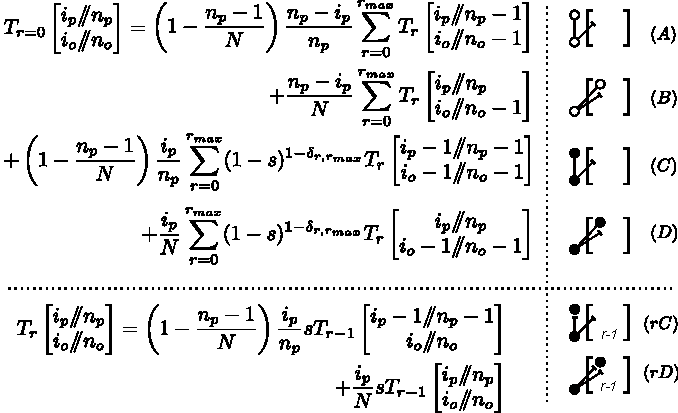
\includegraphics[width=0.9\textwidth]{fig/recurrence-selection-dynamic-failures-annotated.pdf}

  \caption{Recursion construct for transition probability with selection, accounting for multiple
    kinds of coalescent events. The right hand panel represents summands on the left graphically.
    Filled and empty circles represent derived and ancestral alleles. Solid and broken lines are
    successful lineage draws and re-draws due to selection. Double lines represent potnetially
    multiple draws. Square brackets represent events in a smaller sample size ($n_o-1$). Summands
    (\textit{A-D}) are successful draws where the last lineage is ancestral (\textit{A,B}) or
    derived (\textit{C,D}). Note that these terms depend on the probability that there were between
    $0$ to $r_{max}$ in sample size $n_o-1$. Terms \textit{rC} and \textit{rD} represent the
    probability that last selection re-draw was due to a lineage from outside (\textit{rC}) or
    within (\textit{rD}) the sample. See table XX for notation used. }

  \label{fig:rec-selection-dynamic-fail}
\end{figure}
 
There are other ways to write down similar recursion equations. In the appendix, we show a simpler
model for neutral alleles, and a more direct model where $r_{max}=1$.

Using a dynamic programming algorithm, we implement the construction of the exact neutral transition
matrices $\mathbf{T}$ in $O(n^3)$ operations. The set of selection transition probability matrices
$\mathbf{T}$ requires $O(n^4+r)$ operations.

In practice, we set the maximum number of re-draws per lineage to $r_{max}=4$, which appears to be
sufficient to consider strong negative selection up to $Ns=50$.

Since these calculations are expensive, we also propose a number of approximations in the following
sections.


\subsection{Missing probability}

Truncation of the recursion means that some events are not accounted for. Given $j$ derived alleles
in a sample of size $n_o$, probability lost due to truncation is simply $1- \sum_i Q_{n_o}(i,j),$
with the maximum loss of probability occurring for $j= n_o$. Thus the maximum loss of probability
occurs for very deleterious alleles at high frequency -- which is an unusual occurrence. An
alternative method of measuring lost probability is by weighing the missed probability by
$\phi_{n_o}(j)$.


In numerical applications, we re-normalize each row of $Q$ to ensure a proper probability
transition, and we track $1- \sum_i Q_{n_o}(i,n_o)$ to ensure that it remains below a threshold
\sgcomment{What did we use?}.

\section{Results}
\label{sec:results}

% \subsection{Markov process construction}
% \label{subsec:markov}

% \sgcomment{Do we really need the following two paragraphs?}

% The sample size $n_o$ can range between $1$ and $N$, the size of the entire population. We expect that 
% when $n\ll N$, the calculations with the present model do not differ substantially from the
% prediction under the standard coalescent, or \citep{JouganousEtAl2017}. In the limit where
% $n \ra N$, we expect the transition probabilities in \sgcomment {Call this matrix something else? R? T?} $\mathbf{P}_s$ to approach those in the full
% Wright-Fisher model (\textit{i.e.} \cite[eq. 1.58]{Ewens2004}).

% Similar to \eqref{eq:op-selection}, the transition probability matrix with selection
% ($\mathbf{P}_s$), involves considering a large number of intermediate lineages. In practice, we
% limit the number of selective events to at most one per lineage -- which means that the maximum
% number of contributing lineages is $2n_o$ -- one selective death for each offspring. This allows us
% to model strong selection, while limiting the number of coalescent configurations we need to
% consider when building $\mathbf{P}_s$. 

\subsection{Calculation of allele frequency spectra}
\label{subsec:afs}

Once the truncated matrix $\mathbf{Q}_s$ is constructed, it can be used to calculate the allele
frequency spectrum. For example, in the infinite sites model at equilibrium, we can approximate the
equilibrium \textit{AFS} $\Phi$ as a solution to a linear system:

\begin{equation}
  \label{eq:sfs-calc}
  \Phi = Q \Phi  + n \mu e_1
\end{equation}

where $\mu$ is the per-site mutation rate, and $e_1$ is the first column of the identity matrix of
size $n$. Figure \ref{fig:strong-selection} shows the comparison of the \textit{AFS} calculated from
Equation \eqref{eq:coal-recursion, eq:sfs-calc}, the diffusion approximation \cite[eq.
9.23]{Ewens2004}, and the calculation performed in \texttt{Moments} \citep{JouganousEtAl2017}.
\sgcomment{Should we give an example for very large sample sizes on panels A and B to show the
  finite sample effect?} \ikcomment{Is $n=100, N=100$ good here?}. Panels A and B show the
\textit{AFS} under neutrality, C and D under strong negative selection. Under neutrality, all the
models agree, yeilding similar \textit{AFS}.

Figure \ref{fig:strong-selection}C shows a comparison at strong negative $Ns=50$, with the
population size ($N=1000$), which is substantially larger than the sample size ($n=100$). There is a
small deviation between the approaches at large allele frequencies. If the sample size is the same
as the population size ($n=N=100$) (Fig. \ref{fig:strong-selection}D), the diffusion approximation
and \texttt{Moments} depart from the Wright-Fisher prediction. The approach presented here
(\ref{eq:coal-recursion}) shows a better match to the Wright-Fisher model.

\begin{figure}
  \centering
  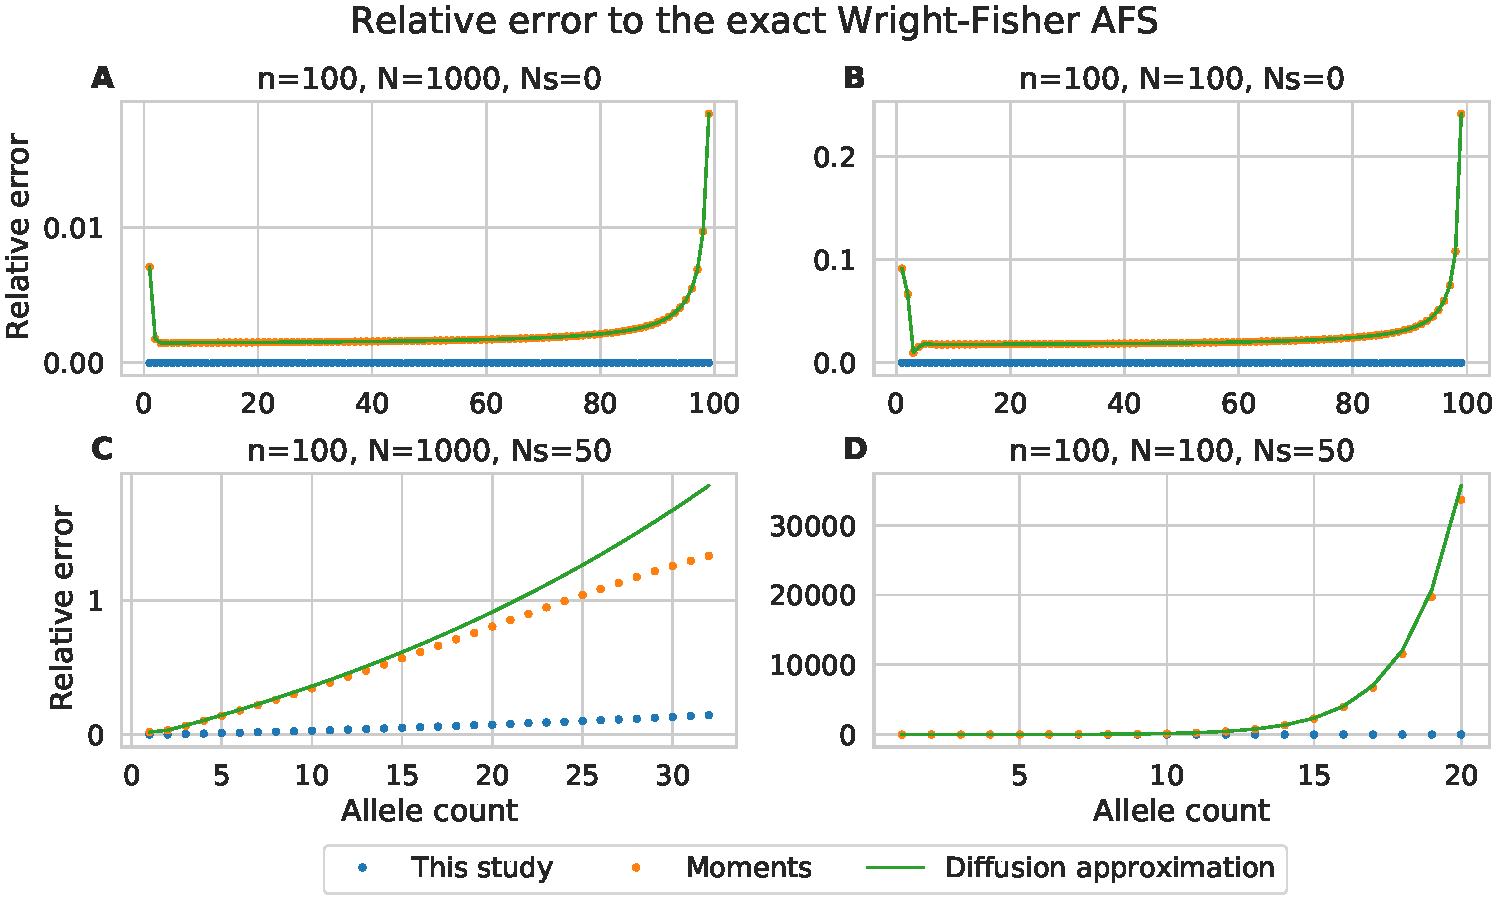
\includegraphics[width=0.7\textheight]{fig/strong_selection_four_panel.pdf}
  \caption{Normalized allele frequency spectra in a sample of size $n=100$ (B,D), for neutral (Ns=0)
    (A,B), or highly deleterious alleles ($Ns=50$) (C,D). (A) shows the frequency spectrum in a
    sample from a large population ($N=1000$), (B) in a small population ($N=100$). (C,D) same, for
    deleterious allele. Note that for a strongly deleterious allele, the probabilities are extremely
    small.
    \label{fig:strong-selection}
   }
 
\end{figure}

\subsection{Closure properties}
\label{subsec:closure}

\sgcomment{I added the closure derivation higher up. So here we can focus on the results. }

To investigate the closure properties of $\mathbf{P}_s$, we can calculate the total probability that
more that $n_o$ parental lineages contribute to a sample of size $n_o$. \sgcomment{I'm not sure
 I understand what you describe below. My take:}
Since $P_{n_o,n_p}(i,j)$ is a probability distribution over $n_p$ and $i$, we can easily compute the probability lost to 
truncation as $1-\sum_{i=0}^{n_o} \sum_{n_p=0}^{n_o}{P_{n_o,n_p}(i,j)}$. 


By construction, the sum
of rows of $\mathbf{P}_s$ should correspond to the total probability mass that included
configurations contribute (Fig. \ref{fig:rec-selection}). Thus, the probability that some number of
configurations are unaccounted for, with $j$ derived alleles in the parental sample, is given by
$1-\sum_{i=0}^{n}\mathbf{P}_s(i,j)$. This probability depends on the number of derived alleles
carried by the parental sample: the more derived alleles, the higher the likelihood of a selective
event. Figure \ref{fig:missing} shows the probability of missing configurations in a sample size of
$n=200$ in the worst-case scenario, with $j=200$ derived lineages.

Since the expected number of drift events increases quadratically and the number of selective events
increases only linearly, the probability that we need additional lineages decreases rapidly with
sample sizes.

\section{Asymptotic closure properties}
\label{sec:asympt}

We now want to determine what sample size is sufficient so that the number of coalescent events due
to drift is almost always larger than the number of selection events, such that the system remains
closed \eqref{eq:op-selection}. We derive several approximations to the model proposed in the first
section, in order to get a better understanding of this behavior.

In the following derivations, we are assuming that the derived allele is present at frequency $x$,
as opposed to explicitly modeling the count of derive alleles \ref{sec:markov}, which simplifies the
calculations. When looking for the upper bound on the number of rejected lineages, we take $x=1$,
since only derived alleles experience selection.

\subsection{Mean number of contributing lineages}
\label{sec:mean-contr}


For a given sample size, the probability that $n_p$ parents have contributed is:

\begin{align}
  \label{eq:conditional}
  Pr(n_p | n_o) = \sum_{n_g} Pr(n_p | n_g)Pr(n_g | n_o)
\end{align}

Where $n_p$ and $n_g$ is the number of contributing parents and gametes, respectively (Fig.
\ref{fig:schematic}B). %Note that we consider this backward in time, so $n_o$ is given, and we ask
%the probability of $n_p$ conditional on $n_o$.

Using the law of total expectation, we can write the expectation $E[n_p-n_o | n_o]$ as 
\begin{equation*}
  \begin{aligned}
    \label{eq:lineages-approx}
    E[n_p -n_o | n_o] &= E[n_p | n_o] - n_o \\
    &=E_{n_g} E_{n_p}[n_p | n_g] -n_o.
  \end{aligned}
\end{equation*}
Assuming $x=1$, the expectation over $n_p$ simply given by the occupancy distribution \cite{}. 

\begin{equation*}
  \begin{aligned}
    \label{eq:lineages-derive}
    \hat{E}[n_p -n_o | n_o] & =   E_{n_g}\left[N\left[1-\left( 1 - \frac{1}{N} \right)^{n_g} \right]\right]- n_o\\
    & =   N-N  E_{n_g}\left[\left( 1 - \frac{1}{N} \right)^{n_g} \right] -n_o. 
  \end{aligned}
\end{equation*}

Since $n_g-n_o$ follows a negative binomial distribution with $n_g$ trials and success rate $1-s$, we can use the moment generating function to show that for any constant $x$,

\begin{equation}
E_{n_g}[x^{n_g}] = x^{n_o}  \left(\frac{1-s}{1-sx}\right)^{n_o}.
\label{eq:identity}
\end{equation} 

Thus we can write 
\begin{equation*}
  \begin{aligned}
    \label{eq:lineages-exact}
    \hat{E}[n_p -n_o | n_o]    & =   N-N  \left( 1 - \frac{1}{N} \right)^{n_o}\left( \frac{1-s}{1-s \left( 1 - \frac{1}{N} \right)}\right)^{n_o}     -n_o.
  \end{aligned}
\end{equation*}

Taking the terms of order $\frac{1}{N}$ gives

\begin{equation*}
    \label{eq:lineages-approx}
    \hat{E}[n_p -n_o | n_o]    =   n_os - \frac{n_o (n_o-1) }{2N}  
\end{equation*}

We thus have the usual result that the increase of the number of lineages due to selection is
linear, whereas the reduction due to drift is quadratic. Solving for $ \hat{E}[n_p -n_o | n_o]<0$ yields, to leading order,

\begin{equation}
  \label{eq:critical-sample}
  n_o^* \ge 2Nxs.
\end{equation}

Figure \ref{fig:critical-sample-size} shows the critical sample size for several selection
coefficients, assuming the entirety of the sample is derived ($x=1$) in a population of $N=1,000$.
The $Y$ axis shows the fraction of contributing parental lineages to the sample size,
$\frac{n_p}{n_o}$. Above the horizontal line $\frac{n_p}{n_o} > 1$, selection dominates. Below,
drift reduces the number of used lineages. The intercept of the line with $\frac{n_p}{n_o} = 1$ is
the critical sample size, which is well-approximated by $2Nsx$.

\subsection{Distribution of number of contributing lineages}
\label{subsec:distribution}

To ensure approximate closure of the recursion, we need a stricter constraint, that is,
$n_p\leq n_o$ almost always (rather than on average. We therefore need to study the distribution
$P(n_p|n_0)$.

We can obtain the variance of this distribution by using the law of total variance:

\begin{equation}
\Var\left[n_p-n_o \right] = \Var_{n_g}\left[E\left[n_p-n_o | n_g \right]\right]+  E_{n_g}\left[Var\left[n_p-n_o | n_g \right]\right] 
\end{equation}

The expectation in the first term can be derived from the occupancy distribution and the identity \ref{eq:identity}:

\begin{equation}
\begin{split}
\Var_{n_g}\left[E\left[n_p-n_o | n_g \right]\right] &= \Var_{n_g}\left[E\left[n_p| n_g \right]\right] \\
&= \Var_{n_g}\left[N\left(1-(1-\frac{1}{N})^{n_g} \right) \right] \\ 
&= N^2 \Var_{n_g}\left[(1-\frac{1}{N})^{n_g} \right] \\
&= N^2 \left( E_{n_g}\left[(1-\frac{1}{N})^{2n_g} \right] - E_{n_g}\left[(1-\frac{1}{N})^{n_g} \right]^2\right) \\
&= N^2 \left( \left(1-\frac{1}{N}\right)^{2n_o} \left(\frac{1-s}{1-s  \left(1-\frac{1}{N}\right)^2}\right)^{n_o} 
-   \left(1-\frac{1}{N}\right)^{2n_o} \left(\frac{1-s}{1-s  \left(1-\frac{1}{N}\right)}\right)^{2n_o} \right) \\
\end{split}
\end{equation}

The variance of the second term is the variance of the occupancy distribution \cite{}:

\begin{equation}
\begin{split}
E_{n_g}\left[Var\left[n_p-n_o | n_g \right]\right] & = E_{n_g}\left[N ((N - 1) (1 - 2/N)^{n_g} + (1 - 1/N)^{n_g} - N (1 - 1/N)^{2 n_g}) \right] \\
& = N (N-1)  \left(1-\frac{2}{N}\right)^{n_o} \left(\frac{1-s}{1-s  \left(1-\frac{2}{N}\right)}\right)^{n_o} +  \left(1-\frac{1}{N}\right)^{n_o} \left(\frac{1-s}{1-s  \left(1-\frac{1}{N}\right)}\right)^{n_o} \\
&-N  \left(1-\frac{1}{N}\right)^{2n_o} \left(\frac{1-s}{1-s  \left(1-\frac{1}{N}\right)^2}\right)^{n_o}. 
\end{split}
\end{equation}

The two terms can be put together to provide an analytical expression for the variance of $n_p$. 




The number of parental lineages used by drift can be modelled by the modified occupancy
(Arfwedson) distribution \citep{Wakeley2009,ONeill2019,JohnsonEtAl2005}. This is given by:

\begin{align}
  \label{eq:occupancy}
  P(n_p|n_g) = \frac{S_2(n_g,n_p) N!}{(N-n_p)! N^{n_g}}
\end{align}
where $S_2(n_g,n_p)$ is a Stirling number of the second kind, which is the number of ways to partition
$n_g$ gametes into $n_p$ parents (see \cite{JohnsonEtAl2005} section 10.4 for a thorough treatment).
Note that the under drift, the number of parents will be smaller or equal to the number of gametes
$n_p \le n_g$.

The distribution of the number of gametes, $n_g$ is given by the negative binomial, parameterized by
probability of resample $s$, and the total number of trials before $n_o$ successes (\textit{i.e.}
$n_r+n_o$):

\begin{align}
  \label{eq:neg-binomial-trials}
  P(n_g|n_o) = \binom{n_g-1}{n_o-1}(1-xs)^{n_o}(xs)^{n_g-n_o}
\end{align}

Here, the number of gametes can be larger that the sample size $n_o \le n_g$, if selection is present.

Combining the two distributions together through \ref{eq:conditional}, we get:

\begin{align}
  \label{eq:lineages-in-past}
   Pr(n_p|n_o) = \sum_{n_g=1}^{\infty} \frac{S_2(n_g,n_p) N!}{(N-n_p)! N^{n_g}} \binom{n_g-1}{n_o-1}(1-xs)^{n_o}(xs)^{n_g-n_o}
\end{align}

This distribution does not appear to have a simple analytical form. However, it can be computed
efficiently using methods presented in \citep{ONeill2019}. Figure \ref{fig:sampling-dist} shows the
distribution of the number of contributing parental lineages for several selection coefficients for
a sample $n=20$. In the absence of selection, the distribution has zero probability above $n=20$, as
no extra lineages can be sampled. As the strength of selection is increased, we begin requiring
larger number of lineages.

\begin{figure}
  \centering
  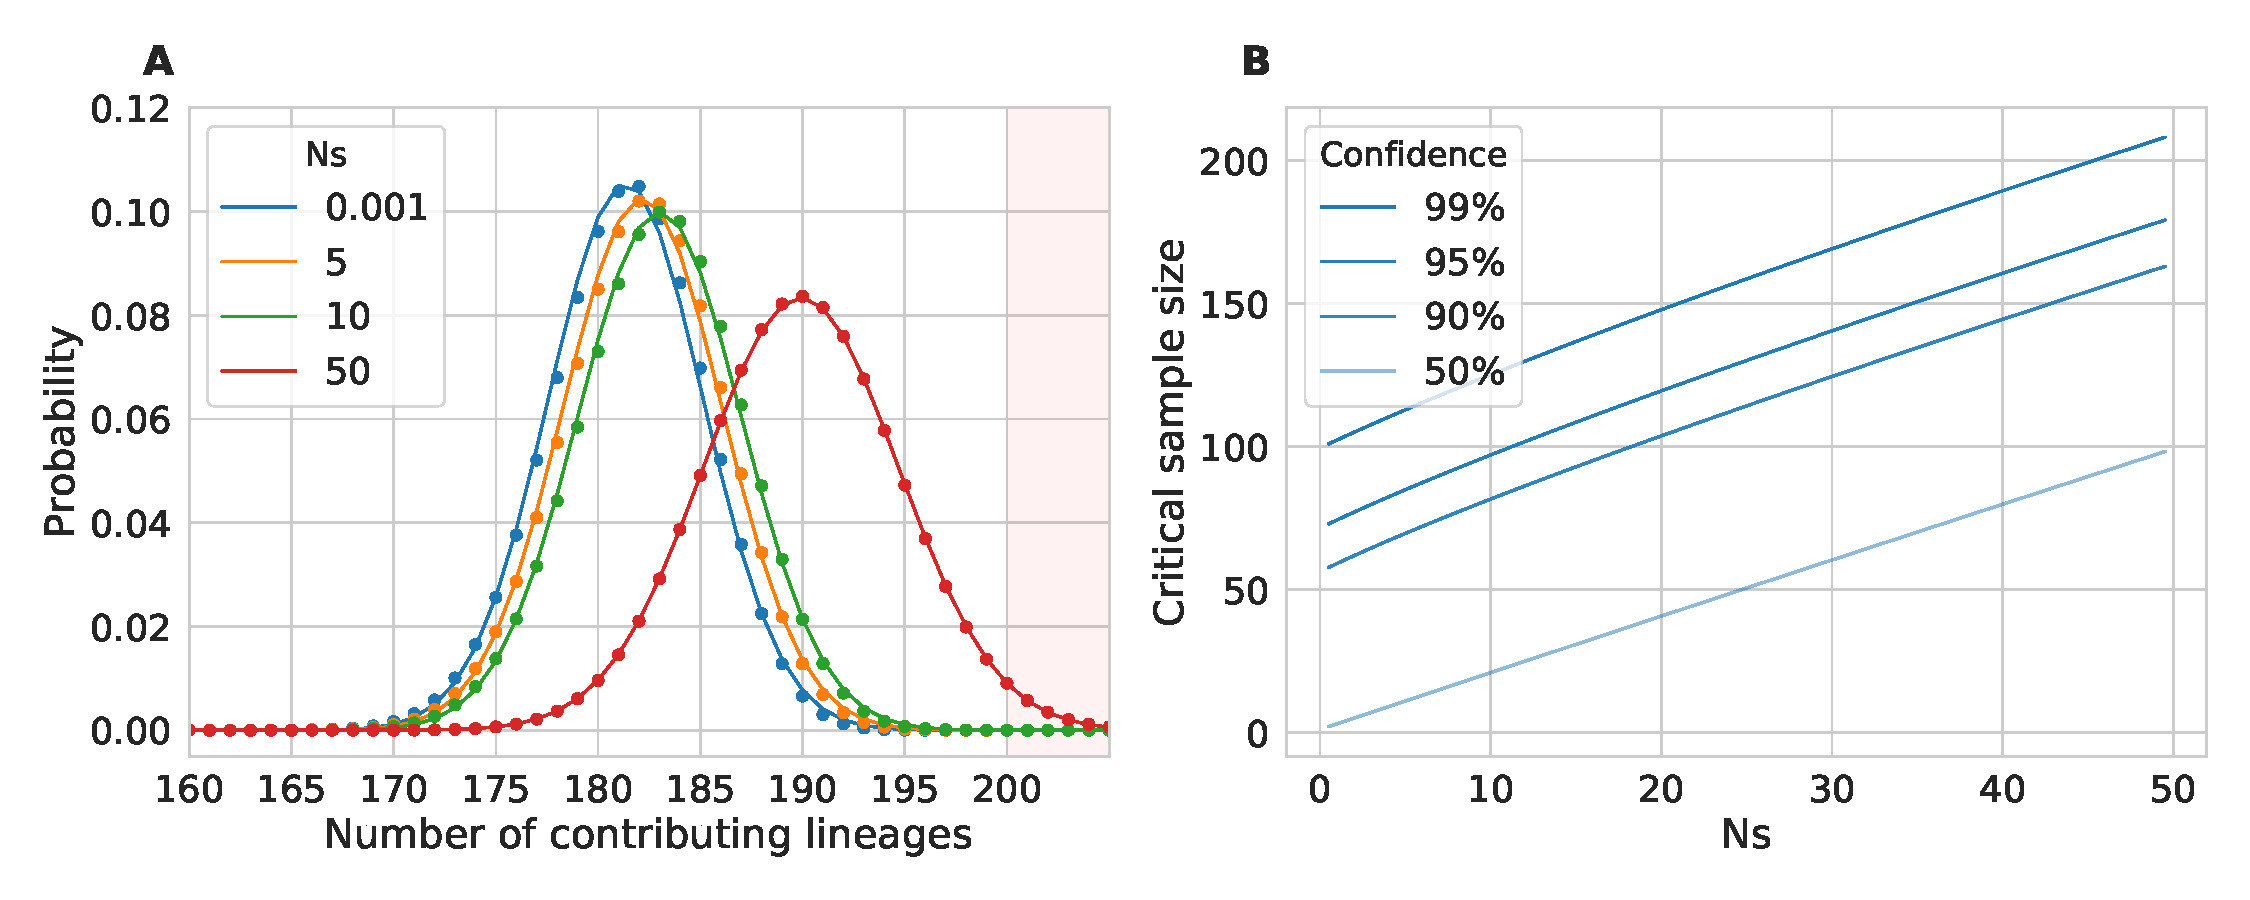
\includegraphics[width=\textwidth]{fig/combined.pdf}
  \caption{\textbf{A} The distribution of number of required lineages, \textbf{B} critical sample
    size to contain all lineages, with given confidence ($n=200$, $N=1000$). Shaded red area shows
    missing probability.}
  \label{fig:combined}
\end{figure}

We defined the critical sample size as $n_o^* > E[n_p | n_o]$. However, the distributions in
\ref{fig:sampling-dist} show that there is a large probability that $n_p>n_o$ at $n_o^*=2n=20$. In
order to guarantee that drift will out-pace selection, we can calculate the cumulative distribution.
This implies that a sample size in which the \textit{majority} of lineages are accounted for can be
substantially larger than the critical sample size of equation \eqref{eq:critical-sample}. To derive
a convenient analytical approximation, we turn to the normal approximation in the next section.

\subsection{Normal approximation}

We can construct a normal approximation to the distribution of the number of contributing lineages.
This approximation will allow us to calculate sample size where, for example, the number of
contributing lineages is smaller that the sample size $95\%$ of the time, instead of $50\%$, as
given by $n_o^*$ in equation \eqref{eq:critical-sample}.

The occupancy distribution is approximated by the normal \citep{ONeill2019} when $n_o \ll N$.
Likewise, the number of failures ($n_r$) before a given number of successes, can be approximated by
the normal distribution. In the case of large population size, as required by the approximation of
the occupancy by the normal, we can approximate the total number of contributing lineages as the sum
of lineages contributed by the two distributions.

The random variable which is a sum of two normally-distributed random variables is also normal, with
$\mu=\mu_1+\mu_2$ and $\sigma^2 = \sigma^2_1 + \sigma^2_2$. By combining the required expectations
and variance, we find that the normal approximation then has the form:

\begin{align}
  \label{eq:normal-approximation}
  Pr(\mathcal{R}=r|n) \approx \mathcal{N}( \mu &= \left[(s n)/(1 - s) + N (1 - (1 - 1/N)^n)\right],\\
  \sigma &= \sqrt{N \left((N-1) \left(1-\frac{2}{N}\right)^n+\left(1-\frac{1}{N}\right)^n-N\left(1-\frac{1}{N}\right)^{2 n}\right)+\frac{n s}{(1-s)^2}})
\end{align}

Figure \ref{fig:normal-approximation} shows the quantiles of the normal approximation. We see that
up to $99\%$ of the lineages will be contained within the sample of 200 with $Ns=20$. Larger
percentiles will require larger sample sizes.

\subsection
{Integrating over few generations} 
To increase the chances that the number of lineages ancestral to a sample 
of size $n_o$ is less than $n_o$, we can also chose to compute a transition matrix over more 
than a single generation. In this case, lineages gained by selective death at one generation can 
can be compensated by loss to genetic drift at another generation. If the expected number of 
drift events is higher than the expected number of selective deaths, this can reduce the likelihood 
of chance events. Asymptotic results suggest ... 

Such transition matrices can also be computed iteratively. If  $n_g$ is the number of contributing 
lineages in the grandparental generation, and $k$ is the number of derived among those, and we define 
 $P(i, n_g | q(k, n_g))$, as above, as the probability of drawing $i$ derived alleles and using exactly $n_g$
 grandparental alleles given the event $q(k, n_g)$ $k$ of the first $n_g$ grandparental alleles are derived, we can 
 condition on the number of contributing alleles $n_c$ and the number of derived alleles $j$ among them in the parental generation:
 
 \begin{equation}
 \begin{split}
 P(i, n_g | r(k, n_g)) & = \sum_{j,n_c} P(i, n_g ; j, n_c r(j,n_c)  | q(k, n_g))\\
 &= \sum_{j,n_c} P(i, n_c,  r(j,n_c); n_g  | q(k, n_g))\\
 &= \sum_{j,n_c} P(i, n_c|   r(j,n_c); n_g  ; q(k, n_g))  P(r(j,n_c); n_g  | q(k, n_g))\\
 &= \sum_{j,n_c} P(i, n_c |   r(j,n_c))  P( r(j,n_c); n_g  | q(k, n_g))\\
 &= \sum_{j,n_c} P(i, n_c |   r(j,n_c))  P( r(j,n_c); n_g  | q(k, n_g))
 \end{split}
\end{equation}
and \sgcomment{despite the crap notation}, this is just the product of quantities we have already computed.


\section{Conclusion}
\label{sec:conclusion}

Classically, the coalescent considers models in the absence of natural selection. Since selection
can increase the number of contributing lineages back in time, the coalescent can no longer be
represented by trees, but instead acquires a graph structure. The ancestral selection graphs
\citep{KroneNeuhauser1997} deal with this in the limit of large population size ($N$).

The large population size approximation implies that the sample size $n$ is much smaller than the
whole population ($n \ll N$), so it is unlikely that more than one coalescent event will happen per
generation. However, recent work \citep{BhaskarEtAl2014,NelsonEtAl2019} pointed out that this
assumption is unreasonable with sample sizes pertinent to modern experiments. As a results, models
that consider multiple coalescent events per generation are gaining increased relevance in the
field \citep{FlemmingtonVoit}.

In this work we show that increasing the sample size has another unexpected consequence. As sample
size increases, the larger number of lineages needed due to selection can be masked by coalescent
events. In this sense, the large sample size rescues the model from effect of selection. This means
that recursion equations needed to calculate sample properties are asymptotically closed with large
population size.

At first approximation, $n_o^*=2Nsx$ is a critical sample size, where the decrease of lineages due to
coalescent back in time out-competes the increase due to selection (eq. \eqref{eq:critical-sample}).
Further, we derive the full probability distribution for the number lineages needed with given
selection coefficient and sample size (eq. \eqref{eq:lineages-in-past}). Unfortunately, the
distribution does not have a closed form, so we derive a normal approximation to the number of
lineages that contribute to a sample (eq. \eqref{eq:normal-approximation}). The normal approximation
then allows us to get a quantile function that we use to find if the model preserves closure with
some confidence level.

This work has several implications. First, we can combine the model described here with the
jackknife approximation \citep{JouganousEtAl2017}. This will allow us to construct a more robust
inference framework that can account for large sample size and strong selection.

Further, the results here suggest that effect of weak selection may be detectable in studies with
large sample sizes. This may open up a way for new investigations of natural selection in population
genetics.

\bibliography{disco}

\section{Appendix}
\subsection{Table of symbols}

\label{ssec:tab-symbols}
\begin{center}
\begin{tabular}{lll}
Symbol & Generation & Meaning\\
\hline
$p$ & $t-1$ & Parental generation\\
$c$ & $t-\frac{1}{2}$ & Contributing (intermediate, selection only)\\
$o$ & $t$ & Offspring (current) generation\\
\end{tabular}
\end{center}

\begin{center}
\begin{tabular}{ll}
Symbol & Meaning\\
\hline
$n$ & Sample size\\
$i$ & Number of derived alleles in sample $n_{\cdot}$\\
$\Dfrac{i}{n}$ & $i$ derived \emph{out of} $n$ total alleles\\
\end{tabular}
\end{center}

\subsection{Neutral case}

We want to construct the entries in the probability matrix
$P\left[ \Dfrac{\cdot}{n_o} \cond \Dfrac{\cdot}{n_p} \right]$ in terms transition probabilities in
smaller sample sizes. Under neutrality, the number of contributing parental lineages $n'_p$ (at
$t-1$) can not be larger than the number of offspring lineages $n_o$. Since $\mathbf{P}$ is square,
$max(n_p)=max(n_o)=n$. Thus, our aim is to express every entry of $\mathbf{P}$,
$P\left[ \Dfrac{\cdot}{n} \cond\Dfrac{\cdot}{n} \right]$, in terms of
$P\left[ \Dfrac{\cdot}{n-1} \cond \Dfrac{\cdot}{n-1} \right]$. Since we never require extra lineages
($n_p\le n_o$), the recurrence is closed.

To calculate the transition probabilities, we first condition on the state of the last parental
allele drawn, and then on the coalescent event that last offspring lineage participates in. The
recurrence is shown in figure \ref{fig:rec-neutral}. The panel on the right depicts the coalescent
event for each term. Empty circles represent ancestral alleles, filled circles -- derived. The
square box represents a sample of size $n-1$. The first three terms in the sum correspond to the
cases where the last parent that we drew was ancestral, last three -- derived.
\sgcomment{Would it be worth presenting the non-square transition probabilites as well to prepare the reader for what comes next with selection}

\begin{figure}
  \centering
  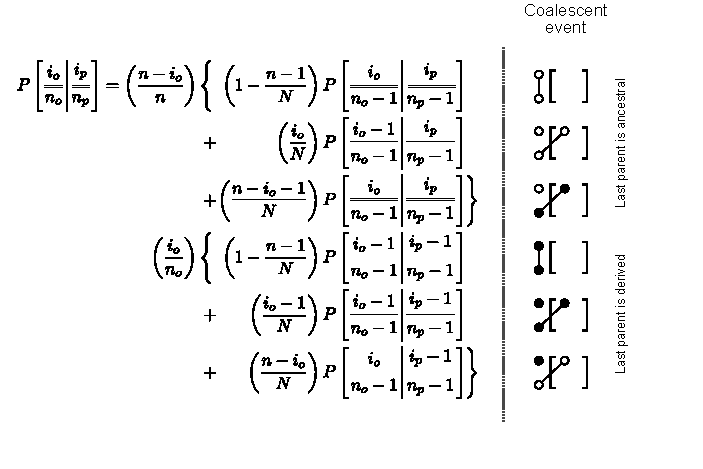
\includegraphics[width=0.9\textwidth]{fig/recurrence-neutral-annotated.pdf}
  \caption{Recurrence defining transition probabilities in a model without selection. Right panel
    shows coalescent events corresponding to each summand. Each transition probability is defined in
    terms of transition in a smaller sample size. First three terms are conditional on the last
    parent having an ancestral state, last three -- derived. Filled circles -- derived alleles;
    empty circles - ancestral alleles; square brackets -- sample of size $n-1$.}
  \label{fig:rec-neutral}
\end{figure}

When calculating a single entry in \ref{fig:rec-neutral}, the variables have the following ranges.
\begin{equation}
  \begin{aligned}
    n_p &= n \\
    i_p &\in [0, n] \\
    n_o &= n \\
    i_o &\in [0, n] \\
  \end{aligned}
\end{equation}

The recurrence is calculated while $n>1$, with the following base cases:
\begin{align*}
  P\left[ \Dfrac{1}{1} \cond \Dfrac{1}{1} \right] &= 1 \\
  P\left[ \Dfrac{0}{1} \cond \Dfrac{0}{1} \right] &= 1 \\
  P\left[ \Dfrac{0}{1} \cond \Dfrac{1}{1} \right] &= 0 \\
  P\left[ \Dfrac{1}{1} \cond \Dfrac{0}{1} \right] &= 0 \\
\end{align*}

\subsection{Selection case}

Due to selective deaths, the number of lineages ($n_c$) that contribute to the current generation
can be larger than the number of offspring ($n_o$), and especially so with strong
selection. Because the number of sampling configurations can be large, we use dynamic programming 
to estimate $\mathbf{P}_{n_p,n_o}$ by summing over the possibilities for the last successful draw. Using the
probability interpretation of the transition matrix, $\mathbf{P}_{n_p,n_o}(i,j) = P(i, n_p | r(j, n_p)),$ the
probability that we draw $i$ derived offspring and exactly $n_p$ parental offspring given that $j$ of the first
$n_p$ sampled parental alleles are derived.  The last successful draw event can be specified by the number $t \in \{0,\infty\}$ 
of prior failed draws due to selection since the last successful draw, the allele $a \in {A, D}$ selected, 
and the event $c$ of whether or not the sampled parental allele was previously drawn $c\in \{True, False\}$. We also consider the event $s \in \{True, False\}$ of whether the last draw was successful. Finally, let us define the event $E_{n_o,t}(i,n_p)$ that we have drawn 
$i$ derived offspring among $n_o$ successful draws followed by $t$ failures, and that this required exactly $n_p$ parental lineages.   
\begin{equation}
\begin{split}
P(i, n_p | r(j, n_p)) = P(E_{n_0,0}(i,n_p)  | r(j, n_p)) &=  \sum_{a, c,t} P(a,c,t; E_{n_o,0}(i,n_p)  | r(j, n_p)) 
 \end{split}
\end{equation}
Let us consider the term $a=A$, $c=False$ \sgcomment{We could use a better notation here, eg using tikz. }
\begin{equation}
\begin{split}
P(a=A,c=False,t; E_{n_o,0}(i,n_p)  | r(j, n_p)) &= P(a=A, c=False, t,s=True; E_{n_o,t}(i,n_p-1) | r(j, n_p))\\
&= P(a=A, c=False, t; E_{n_o,t}(i,n_p-1) | r(j, n_p))\\
&=P(a=A, c=False, t ; E_{n_o,t}(i,n_p-1); r(j, n_p-1) | r(j, n_p))\\
&=P(a=A, c=False, t ; E_{n_o,t}(i,n_p-1)| r(j, n_p-1)  r(j, n_p)) P(r(j, n_p-1) |  r(j, n_p))\\
&=P(c=False, t;  E_{n_o,t}(i,n_p-1) | r(j, n_p-1)  r(j, n_p)) \frac{n_p-j}{n_p}\\
&=P(c=False | t;  E_{n_o,t}(i,n_p-1) | r(j, n_p-1)  r(j, n_p)) P(t;  E_{n_o,t}(i,n_p-1) | r(j, n_p-1)  r(j, n_p)) \frac{n_p-j}{n_p}\\
&=\left(1-\frac{n_p-1}{N}\right) P(t;  E_{n_o,t}(i,n_p-1) | r(j, n_p-1)  r(j, n_p)) \frac{n_p-j}{n_p}\\
&=\left(1-\frac{n_p-1}{N}\right) P(t;  E_{n_o,t}(i,n_p-1) | r(j, n_p-1)) \frac{n_p-j}{n_p}
\end{split}
\end{equation}
where the fourth line uses Bayes rule, and  most other lines are exercises in rewriting the same event in different ways. 
Other combinations of $a$ and $c$ also yield expressions in terms of probabilities $P(t;  E_{n_o,t}(i,n_p) | r(j, n_p))$ for the state prior to the successful draw \sgcomment{write down final results?}. 


These can be similarly expressed as recursions over the last draw. Selection only affects derived alleles, but it can occur after both coalescence and non-coalescence events. 
\begin{equation}
\begin{split}
P(t;  E_{n_o,t}(i,n_p) | r(j, n_p)) = \sum_c P(c, t;  E_{n_o,t}(i,n_p) | r(j, n_p)).
\end{split}
\end{equation}

For example, the $c = True$ term can be written as 
 \begin{equation}
\begin{split}
P(c=True, t;  E_{n_o,t}(i,n_p) | r(j, n_p)) &= P(c=True, a=D, s=False, t;  E_{n_o,t}(i,n_p) | r(j, n_p))\\
&= s P(c=True, a=D, t;  E_{n_o,t-1}(i-1,n_p) | r(j, n_p))\\
&= s \frac{j}{N} P( t;  E_{n_o,t-1}(i-1,n_p) | r(j, n_p)),\\
\end{split}
\end{equation}

\sgcomment{I think this might want to be: }
 \begin{equation}
\begin{split}
P(c=True, t;  E_{n_o,t}(i,n_p) | r(j, n_p)) &= P(c=True, a=D, s=False, t;  E_{n_o,t}(i,n_p) | r(j, n_p))\\
&= s P(c=True, a=D, t;  E_{n_o,t-1}(i,n_p) | r(j, n_p))\\
&= s \frac{j}{N} P( t;  E_{n_o,t-1}(i,n_p) | r(j, n_p)),\\
\end{split}
\end{equation}


and similarly for $c=False$ \sgcomment{Write out? TODO, not complete}.  

 \begin{equation}
\begin{split}
P(c=False, t;  E_{n_o,t}(i,n_p) | r(j, n_p)) &= P(c=False, a=D, s=False, t;  E_{n_o,t}(i,n_p) | r(j, n_p))\\
&= s P(c=False, a=D, t;  E_{n_o,t-1}(i,n_p-1) | r(j, n_p))\\
&= s \frac{j}{N} P( t;  E_{n_o,t-1}(i,n_p) | r(j, n_p)),\\
\end{split}
\end{equation}




Putting this all together \sgcomment{pseudocode?}, we can perform an iteration over all $n_o.$ For each $n_o,$  we will compute all terms of the form $P(E_{n_0,0}(i,n_p)  | r(j, n_p)),$ for $i\in\{0,\ldots,n_0\}$, $j\in \{0,\ldots,n_p\}$, and $n_p \in\{1,\ldots,n_{p,max}\}.$ We further need to iterate over the possible number of failed selective events. If we only allow a maximum amount of failed selected events of $t_max$ for each successful draw, the number of terms we must compute is of order $t_max n_p^4$. The number of computations for each term is constant and only depends on previously computed terms. 

To ensure that probabilities do sum to one despite the $t_max$ cutoff, we modify the Wright-Fisher model by imposing a successful draw after $t_max-1$ attempt. Thus terms

$P(a=D,c,t_{max}; E_{n_o,0}(i,n_p)  | r(j, n_p))$ will lose a factor $(1-s)$.   























We use $n_c$, the intermediate number of lineages at time $t-\frac{1}{2}$, which can
potentially be much larger than the number of parents, $n_p$. This is analogous to the gamete
intermediates, as presented in the main text. However, the two are not equivalent, since in this
formulation we apply selection \emph{and} drift on the intermediate lineages. We model the
intermediate contributing alleles as a random sample from $n_p$ alleles, without replacement.

\begin{equation}
  P_s\left[ \Dfrac{i_o}{n} \cond \Dfrac{i_p}{n} \right] = \sum_{i_c,n_c}P_s\left[ \Dfrac{i_o}{n}
    \cond \Dfrac{i_c}{n_c} \right] P_s\left[ \Dfrac{i_c}{n_c} \cond \Dfrac{i_p}{n} \right]
\end{equation}

The probability conditional on the contributing lineages
($P_s\left[ \Dfrac{i_o}{n} \cond \Dfrac{i_c}{n_c} \right]$) is given by equation
\ref{fig:rec-selection}, while $P_s\left[ \Dfrac{i_c}{n_c} \cond \Dfrac{i_p}{n} \right]$ is given by
the hypergeometric distribution. The support of the hypergeometric distribution means that we can
not have $n_c>n$. Note that while $i_c \le n_c \le n$, we can still have $i_c>i_p$ if $i_p$ is
small. A formulation where a $n_c$ is potentially infinitely large will be desirable.

Under the current definition, $P_s$ is not closed, since the cases where $n_c>n$ are not accounted
for. However, as we show in the main text, the formulation is asymptotically closed, as $n$ increases.

The recursive definition in \ref{fig:rec-selection} is analogous to the neutral case, and gives
$P_s\left[ \Dfrac{i_o}{n} \cond \Dfrac{i_c}{n_c} \right]$, the probability that $i_o$ out of $n$
lineages are derived, given that $i_c$ out of $n_c$ contributed to it. To construct this
probability, we condition on the coalescent events involving the last offspring allele. We limit the
model to at most $1$ selective death per lineage. However, in the entire sample, there still can be
a large number of selective deaths. There are 6 distinct coalescent events with $0$ or $1$ selective
deaths, with distinct probabilities based on whether the last offspring allele is ancestral or
derived. This gives 12 different cases:


\begin{figure}
  \centering
  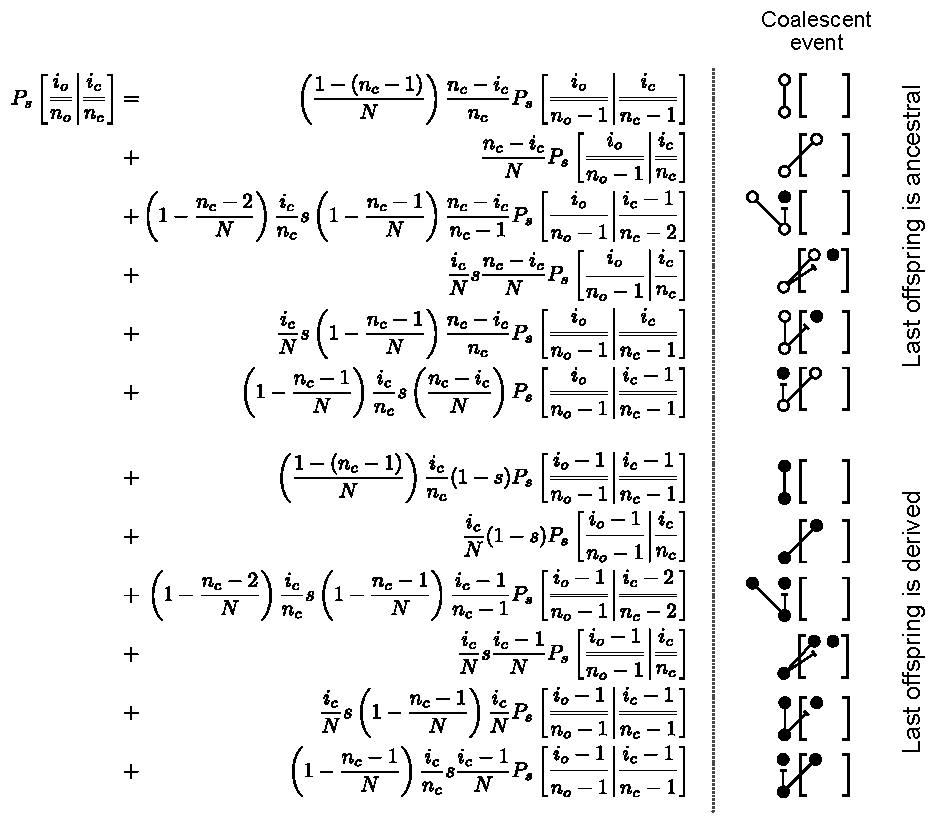
\includegraphics[width=0.9\textwidth]{fig/recurrence-selection-annotated.pdf}
  \caption{Recurrence defining transition probabilities in a model with selection \sgcomment{I think there are some problems with the way fractions are defined, e.g. the first term should start with $1-\frac{n_c-1}{N}$, not $\frac{1-(n_c-1)}{N}$ }. Right panel
    shows coalescent events corresponding to each summand. Each transition probability is defined in
    terms of transition in a smaller sample size. First six terms are conditional on the last
    offspring having an ancestral state, last six -- derived. Filled circles -- derived alleles;
    empty circles - ancestral alleles; square brackets -- smaller sample.}
  \label{fig:rec-selection}
\end{figure}

For each calculation, the ranges of the variables are:

\begin{equation}
  \begin{aligned}
    n_p &= n \\
    i_p &\in [0, n] \\
    n_c &\in [1, n] \\
    i_c &\in [0, n_c] \\
  \end{aligned}
\end{equation}

Note that unlike in the neutral case $n_c$ is now variable. The base cases of the recurrence are:

\begin{equation*}
  \begin{aligned}
    P\left[ \Dfrac{1}{1} \cond \Dfrac{1}{1} \right] &= 1-s \\
    P\left[ \Dfrac{0}{1} \cond \Dfrac{0}{1} \right] &= 1 \\
    P\left[ \Dfrac{1}{1} \cond \Dfrac{2}{2} \right] &= s \\
    P\left[ \Dfrac{0}{1} \cond \Dfrac{1}{2} \right] &= \frac{1}{s} \\
    \text{otherwise} &\phantom{{}=} 0
  \end{aligned}
\end{equation*}

\end{document}
